\chapter{少资源微调——少样本微调的能力激活与知识激活}

前文讲述了大规模预训练过程中,使用可预测预训练技术能使训练变得高效。从本章开始,将讲述在微调方向上的高效训练尝试。微调上的挑战包括数据上的高效性和存算资源的高效性。本章将对少资源微调之一——少样本微调进行初步探索。本文提出预训练过的模型本身可以进行少样本学习,利用能力激活和知识激活技术可以更高效的激发模型预训练时获得的能力和知识,从而需要更少的样本来完成下游任务。本节中的预训练模型,指仅仅经过预训练阶段,未经过指令微调的模型。


\section{基于能力激活的少资源微调初探}

\subsection{背景}
近年来,预训练语言模型~\cite{lewis-etal-2020-bart, han2021pretrained, raffel2020exploring, brown2020language} 在各种任务中取得了显著的性能提升,甚至在语言能力基准测试中超越了人类水平~\cite{wang-etal-2018-glue, wang2019superglue,srivastava2022beyond}。预训练语言模型的这种前所未有的能力为各种实际应用奠定了基础。例如,展现了一般世界知识和常识知识的预训练语言模型是后续成为通用问答模型的核心组件~\cite{tafjord2021general,guu2020retrieval}。

\begin{figure}[!htpb]
    \centering
    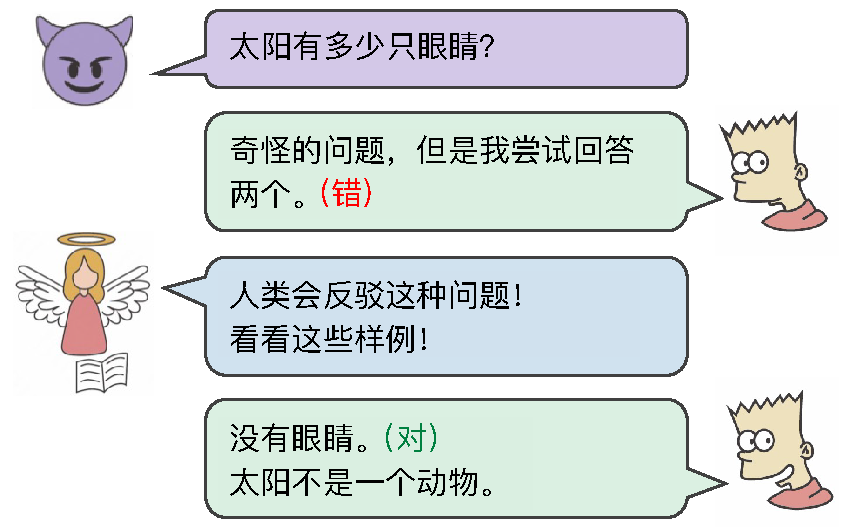
\includegraphics[width=0.8\linewidth]{fpqafigs/intrograph_v4.zh.pdf}
    \caption{预训练模型的反驳能力能通过人工标注的反驳示例激活}
    \label{fig:intrograph}
\end{figure}

\begin{table}[]
    \centering
    \caption{一些先前的研究指出了预训练模型面对误导性问题的脆弱性}
    \resizebox{0.75\linewidth}{!}{
        \begin{tabular}{m{5.8cm}|m{3.3cm}}
        \toprule
          问题  & 答案\\
         \hline
         Sally最喜欢的奶牛昨天死了。这头奶牛什么时候会复活?\tablefootnote{\href{https://blog.allenai.org/general-purpose-question-answering-with-macaw-84cd7e3af0f7}{AllenAI博客。}}   & 几天后。 \\
        \midrule
         太阳有多少只眼睛?\tablefootnote{\href{https://lacker.io/ai/2020/07/06/giving-gpt-3-a-turing-test.html}{博客 \textit{Giving GPT-3 a Turing Test}。}}&
         太阳有一只眼睛。 \\
         \bottomrule
        \end{tabular}
    }
    \label{tab:intro_example}
\end{table}

然而,这些基于预训练语言模型的问答模型存在一个有趣的矛盾。一方面,它们在人类提出的正常问题上表现出色。例如,\textsc{UnifiedQA}~\cite{khashabi-etal-2020-unifiedqa} 在许多问答任务中达到了最先进的性能。\textsc{Macaw}~\cite{tafjord2021general} 能够进行多角度问答,并在 Challenge300 数据集~\cite{tafjord2021general} 中正确回答了 75\% 的问题。另一方面,它们在面对具有误导性的问题时表现脆弱(见表~\ref{tab:intro_example})。例如,\textsc{Macaw} 在九个具有误导性的问题中仅正确回答了一个,而包括 GPT-3~\cite{brown2020language} 在内的其他模型则全部失败~\cite{tafjord2021general}。InstructGPT~\cite{ouyang2022training} 也报告称,它无法识别包含错误前提的指令。这些问题对人类来说很容易反驳,但对预训练语言模型却构成了不可忽视的障碍。

如果没有仔细研究,这一矛盾很容易让人得出结论:预训练语言模型缺乏反驳这些问题所需的世界知识或常识知识。尽管预训练语言模型嵌入尽可能多的通用知识至关重要,但本文通过实验发现,预训练语言模型实际上已经具备了处理其失败的那些误导性问题所需的知识(见第~\ref{sec:pilot}节)。因此,本文假设当前预训练语言模型中的知识已经足以处理大部分具有误导性的问题,但如何运用这些知识的能力尚未被激活。

本文提出,可以使用高质量的人类标注数据来对预训练语言模型进行高效的激活。特别地,本文仔细研究了这些具有误导性的问题,这些问题对于预训练语言模型来说属于分布外测试数据。本文通过精心标注一个数据集进行激活,使预训练模型能够泛化到训练数据集之外的误导性问题上。


\subsection{预备知识}
本节介绍错误前提问题(FPQ)的定义,以及关于预训练语言模型在错误前提问题上的初步实验。

\subsubsection{错误前提问题}
在提问时,人类通常假设某些事实是提问者和回答者共同认可的前提。这些事实构成了问题的基础。例如,在问题“太阳有多少只眼睛?”中,问题的目标是眼睛的数量,它假设了“太阳有眼睛”这一事实的正确性。

一般来说,一个事实可以通过关系三元组表示,每个三元组的形式为 \texttt{<主语, 谓语, 宾语>}。一个问题通常是在询问某个关系三元组中缺失的部分。例如,上述问题可以表示为嵌套的三元组 \texttt{<三元组, 数量, ?>},其中 \texttt{三元组 = <太阳, 具有属性, 眼睛>}。本文将完整的关系三元组定义为支持三元组。那么,错误前提问题就是支持三元组不正确的问题。在上例中,\texttt{<太阳, 具有属性, 眼睛>} 在现实背景下是错误的,因此任何基于此三元组的问题都包含错误前提。根据这一定义,“太阳有眼睛吗?”并不是一个错误前提问题,因为它并未假设 \texttt{<太阳, 具有属性, 眼睛>} 为真。事实上,预训练语言模型能够很好地判断此类三元组的真实性,但它们无法回答基于这些三元组的错误前提问题。
\begin{table}[]
    \centering
    \caption{不同模型在错误前提问题上的表现对比}
    \scalebox{0.8}{
        \begin{tabular}{m{2.3cm}|m{1.2cm}|m{5.5cm}|m{1.3cm}|m{4cm}}
        %     \begin{tabular}{c|c|c|c|c}
        \toprule
          模型 & 参数量 & 生成答案 & 正确性 & 真实答案 \\
         \midrule
         \multicolumn{4}{c}{\cellcolor[HTML]{EAEAEA} 老虎的蛋比鸡蛋大吗?} &\cellcolor[HTML]{EAEAEA} 老虎会下蛋吗?\\
        % \multicolumn{4}{c}{ 你最喜欢哪部中国经典,浮士德还是哈姆雷特?} &浮士德和哈姆雷特是中国经典吗?\\
         \midrule
          Bloom & 176B &  不,老虎的蛋比鸡蛋小... & \xmark & 老虎不会下蛋。\\
          OPT & 175B & 是的。 & \xmark & 不,老虎不会下蛋。老虎是哺乳动物。 \\
          Jurassic-1 & 178B  & 不,老虎的蛋和鸡蛋一样大。 & \xmark & 老虎是胎生动物。\\
          GPT-3 & 175B & 是的,老虎的蛋比鸡蛋大。老虎的蛋可以... & \xmark & 不,老虎不会下蛋... \\
          \textsc{Macaw} & 11B & 是的。 & \xmark & 是的。\\ % lyf edit
          \textsc{Macaw}-FPQ & 11B & 老虎不会下蛋,鸡才会下蛋。 & \cmark & 老虎是肉食动物,不会下蛋。 \\ % lyf edit
        \midrule 
         \multicolumn{4}{c}{\cellcolor[HTML]{EAEAEA} 你最喜欢哪部中国经典,浮士德还是哈姆雷特?} &\cellcolor[HTML]{EAEAEA} 浮士德和哈姆雷特是中国经典吗?\\
        % \multicolumn{4}{c}{你最喜欢哪部中国经典,浮士德还是哈姆雷特?} &浮士德和哈姆雷特是中国经典吗?\\
         \midrule 
          Bloom & 176B &   我最喜欢浮士德。我喜欢哈姆雷特,但我最喜欢浮士德。 & \xmark &  不,它们不是。它们是西方经典...\\
          OPT & 175B & 我都喜欢。 & \xmark & 不是。 \\
          Jurassic-1 & 178B  & 我最喜欢浮士德。浮士德是人,哈姆雷特是鬼魂。 & \xmark & 不,它们不是。\\
          GPT-3 & 175B & 我个人更喜欢浮士德,因为它是一部中国经典戏剧... & \xmark & 不,浮士德和哈姆雷特不是... \\
          \textsc{Macaw} & 11B & 浮士德。 & \xmark & 不是。\\ % lyf edit
          \textsc{Macaw}-FPQ & 11B & 浮士德和哈姆雷特是欧洲经典。 & \cmark & 浮士德和哈姆雷特是欧洲经典。\\ % lyf edit
          \bottomrule
        \end{tabular}
    }
    \label{tab:model_comparison}
\end{table}


\subsubsection{预训练语言模型对错误前提问题的原始响应}
\label{sec:pilot}
本文通过一项初步实验验证了预训练语言模型对错误前提问题的响应并不理想,尽管它们具备相关知识。实验使用了 FalseQA 测试集中的问题(见第~\ref{sec:dataset}节),并调用了公开 API 的大型预训练语言模型,包括 Bloom~\cite{scao2022bloom}、OPT~\cite{zhang2022opt}、Jurassic-1~\cite{lieber2021jurassic} 和 GPT-3(text-davinci-003)~\cite{brown2020language}(即 InstructGPT)。实验使用的提示为“\textit{问题:\makebox[6mm]{\hrulefill} 答案:}”,其中空白部分由问题文本填充。表~\ref{tab:intro_example}和表~\ref{tab:model_comparison} 提供了这些模型生成的答案,以及本文模型(\textsc{Macaw}-FPQ )的答案。可以看到,所有模型在这些简单的错误前提问题上都失败了。然而,在“消融”列中,本文惊讶地发现,所有模型对直接询问前提正确性的问题都给出了正确的响应。这促使本文假设,当前预训练语言模型无法处理错误前提问题的原因是反驳能力未激活,而非知识缺失。因此,需要一个专门针对这类能力的高质量人类标注数据集。

\subsection{数据集}
\label{sec:dataset}
构建错误前提问题数据集有两种潜在方法。一种是从自然语料库中收集这些问题。然而,错误前提问题在自然语料库中很少出现,这使得问题收集过程非常费力。其次,即使收集到错误前提问题,这些错误前提是由人类提出的,因此难以被人类检测到,这与本文的研究动机不符。事实上,\citet{min2022crepe} 已经使用这种方法进行了开创性工作。相反,本文的方法是人工编写此类错误前提问题。为确保数据集的质量,本文期望该数据集具备以下关键特征:\textit{广泛覆盖}、\textit{高质量}、\textit{避免捷径} 以及 \textit{对错误前提的详细解释}。下文介绍了确保这些特征的标注步骤。

\subsubsection{错误前提问题的分类}
人们在不同上下文和形式中提出问题。增加问题的覆盖范围已被证明是有益的\cite{khashabi-etal-2020-unifiedqa}。然而,让标注者自由编写错误前提问题并不能保证问题的覆盖范围。因此,本文手动构思了 29 个初始错误前提问题,然后根据错误类型和问题形式对这些问题进行分类。表~\ref{tab:error_types} 总结了这些分类。总共有八种错误类型,涵盖常识错误、逻辑错误等,以及六种问题形式,涵盖事实性问题、描述性问题等。尽管本文尽可能多地收集了初始示例,但这些分类远未穷尽。因此,本文加入了“其他”选项以鼓励创造性。

\textbf{编写错误前提问题。} 本文招募了二十名人类标注者来构思包含错误前提的问题。为了使创作过程更简单,本文为标注者提供了源词以组成句子。本文使用 GenericsKB~\cite{bhakthavatsalam2020genericskb} 的主语词作为源词,因为它们覆盖范围广泛,并且每个词都配有一个简短的示例句子,可以启发标注者。然而,本文并不要求标注的句子必须包含源词。此外,标注者可以跳过难以构思的源词。然后,本文要求标注者将问题分类到上述类别中。标注者在完成其部分时需保持类别的平衡分布。对于编写的错误前提问题,本文要求其在语法上正确且包含明显的错误前提。



\begin{figure}[!htbp]
    \centering
    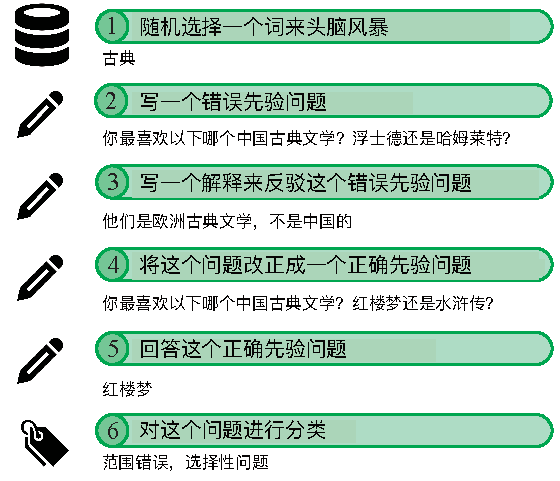
\includegraphics[width=0.7\linewidth]{fpqafigs/annotate.zh.pdf}
    \caption{FalseQA 的标注过程}
    \label{fig:annotateprocess}
\end{figure}

\textbf{修正为正确前提问题(TPQs)。} 先前的研究~\cite{du-etal-2021-towards} 指出,预训练语言模型擅长在数据集中寻找捷径,而并未真正理解任务。由于错误前提问题是人工创建的,很容易陷入标注者的固定写作风格。如果将普通问答数据与标注者数据混合训练,容易被识别出标注者风格的捷径。为了缓解这一问题,本文为这些错误前提问题标注了一个对比集。具体来说,本文要求标注者对每个错误前提问题进行最小程度的修改,使其成为一个具有正确前提的问题(TPQ)。生成的问题对仅在前提的正确性上有所不同,从而确保模型学习到任务的核心。

\textbf{编写详细解释/答案。} 人类通常通过解释前提为何错误来回复错误前提问题~\cite{kaplan1978indirect}。生成解释也有助于检查模型是否真正理解了错误前提问题。因此,本文要求标注者为每个错误前提问题编写解释。为了控制解释的质量,本文要求解释不能仅仅是对错误前提的否定。对于训练集和验证集,每个问题需要一个解释;对于测试集,每个问题需要两个解释。为了对称性,标注者还需为正确前提问题编写答案。完整的标注过程如图~\ref{fig:annotateprocess} 所示。

\begin{table}[]
    \centering
    \caption{错误前提问题的分类及示例}
    \resizebox{0.98\textwidth}{!}{
        \begin{tabular}{m{2.5cm}|c|m{6.5cm}|m{9cm}}
    \toprule
    {\textbf{类别}} & \textbf{占比 (\%)}& \multicolumn{1}{>{\centering\arraybackslash}c|}{\textbf{描述}} & \multicolumn{1}{>{\centering\arraybackslash}c}{\textbf{示例}}\\
    \midrule
    \multicolumn{4}{c}{\cellcolor[HTML]{D0D0D0}{\textbf{错误类型}}}  \\
    \midrule
    属性 & 23.2 & 实体不具备该属性。 & 太阳透明了多久?\\
    \midrule
    行为 & 19.7 & 实体无法执行该行为。 & 鱼能在街上走多远? \\
    \midrule
    范围 & 19.6  & 事实在特定范围内不成立。 & 《冰与火之歌》中与哈利·波特对抗的反派是谁? \\
    \midrule
    实体 & 11.3 & 实体不存在。 & 人类翅膀最常见的颜色是什么?\\
    \midrule
    事件  & 8.3 & 该事件在历史上未发生。 &  扎克伯格何时创立了谷歌?\\
    \midrule
    逻辑 & 6.7& 包含逻辑冲突的陈述。 & 
    如何在走路时坐下? \\
    \midrule
    因果关系  & 5.6 & 不符合因果关系。 & 为什么喝的水越多,越感到口渴?   \\
    \midrule
    索引  & 4.6 & 指定的索引超出实体列表范围。 & 中国第 50 大的省份是哪个?\\
    \midrule
    \multicolumn{4}{c}{\cellcolor[HTML]{D0D0D0}{\textbf{问题形式}}}  \\
    \midrule
    描述性 &  29.6 & 问题需要描述性回答。  & 为什么二氧化碳由氧气组成?  \\
    \midrule
    事实性 & 28.1 &  问题寻求事实性信息。 &  中国何时成为欧盟成员国?\\
    \midrule
    列举性 & 12.3 & 答案是项目列表。 & 列出老虎吃的三种蔬菜。 \\
    \midrule
    选择性 &  10.7 &  提供了答案候选。 & 在剧院中哪种行为是正确的?打架还是扰乱演出? \\
    \midrule
    假设性 & 9.0 & 问题包含条件从句。 & 如果我想看木星上的雾,应该什么时候去? \\
    \midrule
    肯定性 & 8.5 & 问题需要是或否的回答。 &  人们吃钻石是因为它富含多种营养吗? \\ 
    \bottomrule
        \end{tabular}
    }
    \label{tab:error_types}
\end{table}

\subsubsection{数据集统计}
最终的数据集名为 FalseQA,包含 2365 个问题对。表~\ref{tab:FalseQA_examples} 展示了错误前提问题数据集的一个示例。本文随机将数据集按 5:2:3 的比例划分为训练集、验证集和测试集。统计摘要如表~\ref{tab:statisticsofFPQ} 所示。词数通过 NLTK~\cite{bird-loper-2004-nltk} 计算。

\definecolor{greycolor}{rgb}{0.917, 0.917, 0.917}
% \newcolumntype{g}{>{\columncolor{greycolor}}c}



\begin{table*}[!htbp]
    \centering
    \caption{示例问题对及其源词、解释/答案}
    \resizebox{\textwidth}{!}{
        \begin{tabular}{m{2.5cm}|c|m{6cm}|m{6.5cm}}
        \toprule
        源词 & 类型 & \multicolumn{1}{>{\centering\arraybackslash}c|}{问题} & \multicolumn{1}{>{\centering\arraybackslash}c}{解释/答案} \\
        \hline
        \multirow{2}{*}{网球} & 错误前提问题 & 1200 年代网球比赛的举办地点是哪里?& 现代网球在 12 世纪尚未发明。 \\
        & 真实问题 & 2021 年法国网球公开赛的举办地点是哪里?& 2021 年法国网球公开赛于 5 月至 6 月在罗兰·加洛斯举行。 \\
        \midrule
        \multirow{2}{*}{软件} & 错误前提问题 & 列出由爱迪生开发的一款软件。& 爱迪生是物理发明家,而非计算机科学家。 \\
        & 真实问题 & 列出由比尔·盖茨开发的一款软件。& Windows XP。 \\
        \bottomrule
        \end{tabular}
    }
    \label{tab:FalseQA_examples}
\end{table*}

\subsection{实验}
\label{sec:exp}
本文实验分为两个主要部分。首先,通过大量实验证明预训练语言模型在少量训练数据下具备识别和反驳错误前提问题的能力。其次,提出一种实用方法,使模型能够同时处理错误前提问题和一般问题。

\subsubsection{模型与设置}
预训练语言模型通常分为三种主要架构,即仅编码器、仅解码器和编码器-解码器模型。由于仅编码器模型无法直接用于问答任务,本文从后两种架构中选择典型模型进行实验。

对于仅解码器模型,本文选择了 OPT~\cite{zhang2022opt},这是一个与 OpenAI GPT-3~\cite{brown2020language} 对齐的开源预训练模型系列。

对于编码器-解码器模型,本文使用了 T5~\cite{raffel2020exploring} 和 Macaw~\cite{tafjord2021general}。T5 模型通过大规模无监督预训练语料库和多种监督任务进行训练,使其能够解决各种下游任务。Macaw 是基于 T5 模型在问答任务上微调的模型,在直接问答数据集 ARC-DA~\cite{bhakthavatsalam2021think} 上达到了最先进的性能,并在高难度数据集 Challenge300~\cite{tafjord2021general} 的大多数类别上表现良好,但在错误前提问题上表现不佳。

除非特别说明,所有实验均使用不同的随机种子重复三次。对于每个结果,本文报告平均值和标准差。

\begin{table}[!htbp]
    \centering
    \begin{minipage}{0.46\linewidth}
        \centering
        \caption{FalseQA 数据集的统计信息}
        \resizebox{\linewidth}{!}{
            \begin{tabular}{c|c}
            \toprule
            标注者数量 & 20 \\
            错误类型数量(错误前提问题) & 8 \\
            问题形式数量(错误前提问题) & 6 \\
            平均问题长度(错误前提问题) & 10.6 个词 \\
            平均解释长度(错误前提问题) & 12.1 个词 \\
            平均问题长度(正确前提问题) & 10.4 个词 \\
            平均答案长度(正确前提问题) & 9.8 个词 \\
            训练集 & 1187 个问题对 \\
            验证集 & 491 个问题对 \\
            测试集 & 687 个问题对 \\
            \bottomrule
            \end{tabular}
        }
        \label{tab:statisticsofFPQ}
    \end{minipage}
    \hfill
    \begin{minipage}{0.49\linewidth}
        \centering
        \caption{错误前提问题的二分类结果}
        \resizebox{\linewidth}{!}{
            \begin{tabular}{l|c|c|c}
            \toprule
            \multicolumn{1}{>{\centering\arraybackslash}c|}{模型}   & 召回率 &  精确率 & 准确率 \\
            \hline
            OPT-350M & \std{64.8}{7.2} &	\std{65.5}{3.3} &	\std{65.1}{1.8} \\
            OPT-1.3B & \std{67.4}{7.6} &	\std{73.5}{5.1} &	\std{71.2}{0.4} \\
            OPT-2.7B & \std{69.2}{12.2}	&\std{76.7}{5.0} & 	\std{73.7}{2.1} \\
            T5-Large & \std{72.8}{2.3} &	\std{76.9}{1.5}	& \std{75.4}{0.3}  \\
            T5-3B & \std{80.6}{7.7}	& \std{83.8}{4.3} &	\std{82.3}{1.9} \\
            T5-11B & \std{86.5}{1.7} &	\std{82.4}{1.0} &	\std{84.0}{1.1} \\
            \textsc{Macaw}-Large & \std{75.0}{4.1} & 	\std{77.9}{3.3} &	\std{76.7}{0.7}  \\
            \textsc{Macaw}-3B & \std{79.9}{6.8} &	\std{85.0}{5.3} & 	\std{82.6}{0.5} \\
            \textsc{Macaw}-11B & \std{86.0}{2.1} &	\std{87.0}{0.7}	& \std{86.6}{1.3}\\
            \bottomrule
            \end{tabular}
        }
        \label{tab:binary}
    \end{minipage}
\end{table}


\subsubsection{识别错误前提问题}
本文首先训练预训练语言模型将 FalseQA 中的问题分类为错误前提问题(FPQ)和正确前提问题(TPQ)。为了缓解预训练和微调之间的差距,本文采用提示学习范式~\cite{schick-schutze-2021-exploiting,10.1145/3560815} 进行分类。本文报告了分类的准确率,并特别强调了错误前提问题的召回率和精确率。

从表~\ref{tab:binary} 中可以看出,所有模型在二分类任务上均取得了显著性能。

(1) 最强大的模型 Macaw-11B 达到了 86.6\% 的准确率。(2) 对于同类型模型,随着模型规模的增加,性能显著提升。本文假设这种规模效应是因为更大的模型不仅包含更多知识,而且更容易被激活以理解任务。(3) 从 T5 到 Macaw 的性能略有提升,表明通过在正常问题语料库上微调可以增强识别错误前提问题的能力。

\subsubsection{训练数据规模的影响}
本文进一步研究了预训练语言模型在少量训练数据下识别错误前提问题的性能。本文随机抽取了 32、128、256 和 512 对错误前提问题和正确前提问题作为训练数据,并在图~\ref{fig:scale} 中绘制了不同数据规模下的性能。可以看出,随着问题对数量的指数增长,分类准确率几乎呈线性增长。仅需 256 对问题,规模大于 2.7B 的模型(如 OPT-2.7B、Macaw-3B 和 Macaw-11B)均能达到 70\% 以上的准确率,而较小模型则需要更多数据才能取得显著性能。模型规模与数据规模之间的权衡表明,更大规模的模型可能只需更少的训练数据即可被激活。然而,本文注意到,模型性能与人类性能之间仍存在较大差距,因为普通人几乎可以完全分类此类问题。

\begin{figure}
    \centering
    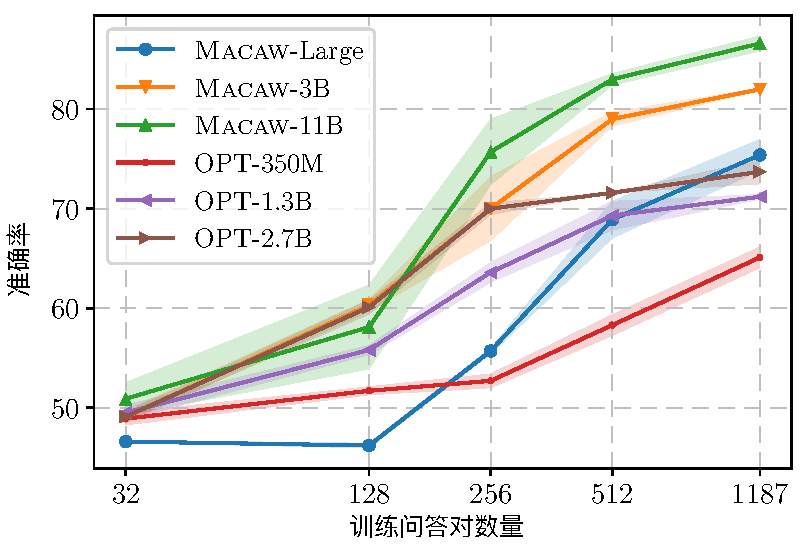
\includegraphics[width=0.67\linewidth]{fpqafigs/exp2.zh.pdf}
    \caption{预训练模型在不同训练样本数量下对错误前提问题的识别能力}
    \label{fig:scale}
\end{figure}

上述结果使本文能够设计一个初步的问答流程来处理错误前提问题。例如,如果模型预测某个问题是错误前提问题,则拒绝回答此类问题,而对于其他问题则生成答案。

\begin{table}[htbp]
    \centering
    \caption{统一错误前提问题的识别与解释生成}
\resizebox{0.65\linewidth}{!}{
    \begin{tabular}{c|l|c|c|c}
\toprule
{问题对} & \multicolumn{1}{>{\centering\arraybackslash}c|}{模型}  & 召回率 & 准确率 & \textsc{Rouge}-L  \\
\hline
\multirow{6}{*}{32} 
& OPT-2.7B & \myemph{\std{62.4}{14.0}} & \std{52.8}{0.7} & \myemph{\std{27.7}{1.9}}  \\
& {\quad{+二元损失}} & \std{59.0}{5.3} & \myemph{\std{56.3}{1.2}} & \std{27.0}{1.6}\\
& \textsc{Macaw}-3B  & \myemph{\std{41.9}{22.3}} & \std{56.8}{3.4} & \std{29.1}{3.0}  \\
& {\quad{+二元损失}} & \std{40.5}{21.8} & \myemph{\std{61.5}{7.7}} & \myemph{\std{32.0}{1.3}}\\
& \textsc{Macaw}-11B & \myemph{\std{64.5}{36.9}} &  \std{59.2}{9.0} & \myemph{\std{36.2}{5.2}} \\
& {\quad{+二元损失}} & \std{49.0}{19.6} & \myemph{\std{64.1}{7.2}} & \std{33.8}{0.5}\\
\midrule
\multirow{6}{*}{256} 
& OPT-2.7B & \std{56.8}{5.3} & \std{56.9}{2.0} & \std{29.5}{0.4} \\
& {\quad{+二元损失}} & \myemph{\std{62.5}{5.5}} & \myemph{\std{67.8}{1.6}} & \myemph{\std{29.7}{0.5}}  \\
&\textsc{Macaw}-3B  &  \std{69.5}{7.5}&\std{73.5}{1.7}&\std{34.5}{1.3}  \\
& {\quad{+二元损失}} &  \myemph{\std{72.6}{8.7}} & \myemph{\std{76.5}{2.3}} & \myemph{\std{35.3}{1.5}} \\
& \textsc{Macaw}-11B  & \std{77.3}{13.0} & \std{76.2}{1.9} & \std{35.0}{2.0}  \\
& {\quad{+二元损失}} & \myemph{\std{81.3}{4.6}} & \myemph{\std{79.2}{0.2}} & \myemph{\std{38.4}{0.7}} \\
\midrule
\multirow{6}{*}{1187} 
& OPT-2.7B & \myemph{\std{76.2}{4.1}} & \std{70.8}{0.9} & \myemph{\std{34.2}{0.6}} \\
& {\quad{+二元损失}} & \std{75.9}{4.9} & \myemph{\std{75.3}{0.5}} & \std{34.0}{1.1} \\
& \textsc{Macaw}-3B  & \myemph{\std{81.8}{7.3}} & \std{80.6}{1.2} & \myemph{\std{39.2}{1.9}}  \\
& {\quad{+二元损失}} & \std{80.9}{1.2} & \myemph{\std{84.2}{0.7}} & \std{38.1}{1.0} \\
& \textsc{Macaw}-11B  & \myemph{\std{90.7}{5.2}} &  \std{83.6}{0.8} & \std{41.9}{0.6}  \\
& {\quad{+二元损失}} & \std{88.8}{1.8} & \myemph{\std{87.1}{0.9}} & \myemph{\std{42.0}{0.7}} \\
\bottomrule
    \end{tabular}
}
    \label{tab:model_stimulation}
\end{table} 


\subsubsection{通过解释回答错误前提问题}
\label{exp:answerfpq}
接下来,本文训练预训练语言模型同时判别错误前提问题并生成解释。由于需要从已经具备零样本问答能力的模型开始,本文仅选择 \textsc{Macaw} 作为编码器-解码器模型。对于仅解码器模型,本文采用与 \citet{tafjord2021general} 类似的方法,使用 UnifiedQA 数据集~\cite{khashabi-etal-2020-unifiedqa} 的一部分训练 OPT 模型,以引导模型进入问答模式,而无需注入大量额外知识。本文选择了能够在使用 256 对数据时取得显著性能的模型规模进行实验。

为了同时判别和生成解释,本文让模型首先生成判别标记:“\textit{误导性问题}”或“\textit{真实问题}”。然后,模型继续生成对错误前提问题的解释或对真实问题的答案。由于负责判别和生成的标记数量差异较大,本文在判别标记上增加了额外的二元损失。二元损失与生成损失的比例为 1。本文在三种训练数据规模(即 32、256 和 1187 对问题)上进行了实验。

在评估中,如果生成的答案包含“\textit{误导性问题}”,则认为该问题被分类为错误前提问题,否则分类为真实问题。与上一节类似,本文报告了预测错误前提问题的召回率、精确率以及二元分类的准确率。此外,本文通过计算生成解释与两个真实解释之间的最大 \textsc{Rouge}-L~\cite{lin2004rouge} 分数来评估生成解释的质量。需要注意的是,由于本文关注的是错误前提问题的解释,评估中不包括真实问题。

表~\ref{tab:model_stimulation} 中展示了结果,其中更好的结果以 \colorbox{emphcolor}{绿色} 标出。 本文得出三个观察结果:(1)模型成功联合预测问题并生成答案;(2)当训练数据有限时(例如 32 对问题),准确率显著高于单独进行分类的情况(见图~\ref{fig:scale}),这表明错误前提问题的解释帮助模型快速适应任务;(3)添加二元损失提高了模型在分类任务上的性能。对于生成的解释,最佳 \textsc{Rouge}-L 分数达到 42.0,表明解释接近人类水平。随着模型规模和数据规模的增加,解释质量也有所提高。

本文在表~\ref{tab:random_sample_10} 中展示了测试集中随机抽样的错误前提问题及其对应的参考解释、分类结果和生成解释/答案。本文使用了经过完整训练数据训练并添加了二元损失的 \textsc{Macaw-11B} 模型进行演示。可以看到,在大多数情况下,模型生成的解释与参考解释接近。然而,也存在生成解释与事实不符的情况。例如,“\textit{蜘蛛的外壳对其呼吸没有帮助}”是不正确的。

\begin{table*}[]
    \centering
    \caption{测试集中随机抽样的错误前提问题}
    \resizebox{\textwidth}{!}{
        \begin{tabular}{c|m{4.5cm}|m{5.5cm}|c|m{5.5cm}}
        \toprule
      编号 &  \multicolumn{1}{>{\centering\arraybackslash}c|}{问题} & \multicolumn{1}{>{\centering\arraybackslash}c|}{参考解释} & 分类结果 & \multicolumn{1}{>{\centering\arraybackslash}c}{生成解释/答案}\\
         \midrule
      1 &  为什么鸟类不是一种动物? & 根据定义,鸟类是一种动物。  &  \cmark & 鸟类是动物。   \\
      2 & 蜘蛛的外壳对其呼吸有帮助吗? & 蜘蛛没有外壳。 & \cmark & 蜘蛛的外壳对其呼吸没有帮助。 \\
    3 & 为什么锂不能燃烧? & 锂容易燃烧并爆炸。 & \xmark & 因为锂是一种金属。\\
    4 & 手杖的脚什么时候生长? & 手杖不是动物,因此没有脚。 & \cmark & 手杖是植物,不是动物,它们没有脚。 \\
    5 & 列出一种有两个耳朵的钟表。 & 钟表不是动物,它没有两个耳朵。  & \cmark & 钟表是机械设备,不是生物,没有耳朵。 \\
    6 & 植物需要多长时间才能长成成年动物? & 植物不会长成成年动物,植物会长成树或更大的植物。 & \cmark & 植物是植物,动物是动物,它们不能长成植物。 \\
    7 & 1350 年的相机是由什么材料制成的? & 相机发明于 1839 年。 & \cmark & 暗箱相机发明于 1839 年。 \\
    8 & 哪个地方有八个季节? & 总共只有四个季节。 & \cmark & 只有四个季节。 \\
    9 & 为什么孕妇有两个肚子? & 孕妇只有一个肚子。 & \cmark & 孕妇只有一个肚子。 \\
    10 & 如果狐狸生活在海里,它们多久上岸一次? & 狐狸没有鳃,不能生活在海里。 & \cmark & 狐狸生活在陆地上。\\
    \bottomrule
        \end{tabular}
    }
    \label{tab:random_sample_10}
\end{table*}


\begin{table}[htbp]
    \centering
    \caption{在不同示例数量下的上下文学习性能}
\resizebox{0.65\linewidth}{!}{
    \begin{tabular}{c|c|c|c|c}
\toprule
{问题对} & {模型}  & 召回率 & 准确率 & \textsc{Rouge}-L  \\
% \multicolumn{5}{c}{\cellcolor[HTML]{D0D0D0}{\textbf{In-context Learning}}}\\
\hline
\multirow{4}{*}{0}& OPT-66B & 6.8 & 25.8 & 12.2 \\
& Jurassic-1  & 66.2 & 36.5 & 6.5 \\
& GPT-3(001) & 46.9 & 46.1 & 5.1\\
& GPT-3(002)  & \myemph{98.5} & \myemph{53.2}  & 
\myemph{25.3} \\
\midrule
\multirow{4}{*}{2}& OPT-66B & \std{21.3}{18.5}&\std{53.0}{2.6}&\std{32.2}{2.8}\\
% \std{21.3}{18.5}&\std{53.0}{2.6}&\std{32.2}{2.8}
& Jurassic-1  & \std{52.8}{37.0}&\std{56.9}{2.6}&\std{32.4}{5.3}\\
% \std{52.8}{37.0}&\std{56.9}{2.6}&\std{32.4}{5.3}
& GPT-3(001) & \std{43.6}{16.7}&\std{63.9}{4.1}&\std{31.8}{2.7}\\
% \std{43.6}{16.7}&\std{63.9}{4.1}&\std{31.8}{2.7}
& GPT-3(002)  & \myemph{\std{87.9}{2.4}} & \myemph{\std{75.2}{1.6}} & \myemph{\std{38.1}{1.5}}\\
% \std{87.9}{2.4}&\std{75.2}{1.6}&\std{38.1}{1.5}
\midrule
\multirow{4}{*}{4} & OPT-66B & \std{19.7}{29.8}&\std{51.9}{3.7}&\std{34.8}{1.4}\\
% \std{19.7}{29.8}&\std{51.9}{3.7}&\std{34.8}{1.4}
& Jurassic-1  & \myemph{\std{94.7}{8.2}}&\std{53.1}{4.8}&\std{38.4}{0.7} \\
% \std{94.7}{8.2}&\std{53.1}{4.8}&\std{38.4}{0.7}
& GPT-3(001)  & \std{61.9}{15.7} &\std{67.6}{1.5}&\std{34.5}{1.2}\\
% \std{61.9}{15.7}&\std{67.6}{1.5}&\std{34.5}{1.2}
& GPT-3(002)  & {\std{90.6}{4.6}} &\myemph{\std{75.8}{2.9}}&\myemph{\std{39.1}{1.6}}\\
% \std{90.6}{4.6}&\std{75.8}{2.9}&\std{39.1}{1.6}
\bottomrule
    \end{tabular}
}
    \label{tab:incontextlearning}
\end{table}


\begin{figure*}[htbp]
    \centering
    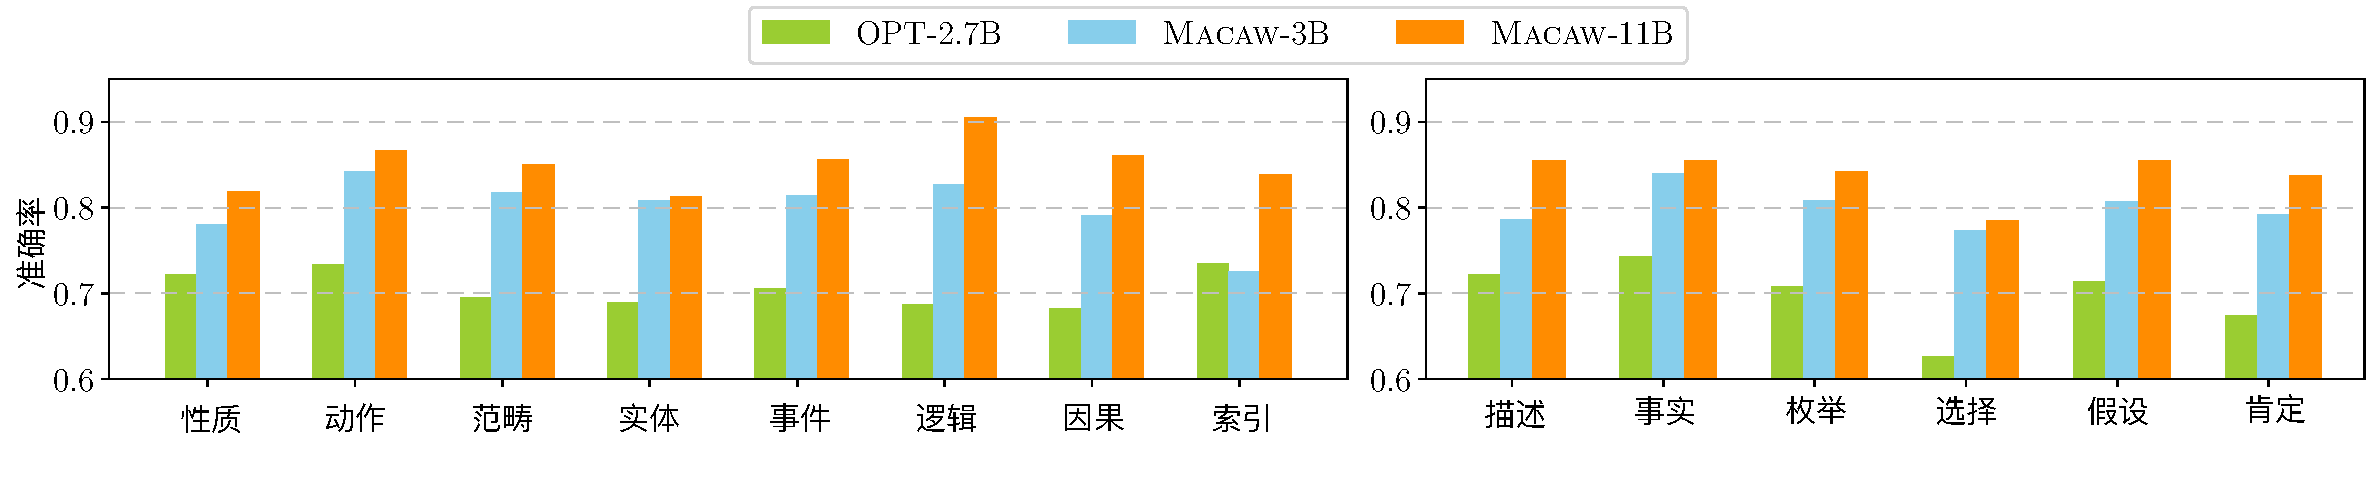
\includegraphics[width=0.97\textwidth]{fpqafigs/category.zh.pdf}
    \caption{预训练模型在不同错误类型和问题形式上的准确率}
    \label{fig:category}
\end{figure*}

\subsubsection{上下文学习(In-context Learning)}
本文进一步研究了更大规模模型(例如 GPT-3)在 FalseQA 上的表现。这些大型预训练语言模型通过上下文学习进行调优,模型参数保持不变。本文选择了 {OPT-66B}~\cite{zhang2022opt}、Jurassic-1~\cite{lieber2021jurassic}、GPT-3(001) 和 GPT-3(002)~\footnote{text-davinci-001 和 text-davinci-002 检查点。}。实验结果如表~\ref{tab:incontextlearning} 所示。更好的结果以 \colorbox{emphcolor}{绿色} 标出。可以看到,OPT-66B 和 Jurassic-1 表现较差。因此,本文得出结论:由于错误前提问题与正常问题的分布不匹配,使用少量示例激活这些模型的反驳能力仍然具有挑战性,这一问题留待未来研究。GPT-3 可以通过 2 或 4 对示例激活,但其性能低于第~\ref{exp:answerfpq} 节中经过微调的小规模模型。令人惊讶的是,GPT-3(002) 的性能远优于 GPT-3(001)。本文假设这是因为 GPT-3(002) 通过指令调优~\cite{ouyang2022training} 训练,更容易理解反驳任务。


\subsubsection{回答错误前提问题与通用问题}
问答模型最初用于回答通用问题,例如 ARC-DA~\cite{bhakthavatsalam2021think}~\footnote{AI2 推理挑战-直接回答(AI2 Reasoning Challenge-Direct Answer)的缩写。} 数据集中的问题,其分布与 FalseQA 不同。因此,仅在 FalseQA 上训练可能会导致灾难性遗忘。为了构建一个能够同时处理错误前提问题和通用问题的模型,本文采用了一种简单的数据回放技术(DR)~\cite{chaudhry2019tiny}。具体而言,在 FalseQA 数据集上训练时,每次迭代批次时,本文会添加一批来自 ARC-DA 的数据样本。为了尽可能少地使用 ARC-DA 数据,本文在 30 次批次迭代内保持 ARC-DA 样本不变。无论是否使用数据回放技术,均采用上述二元损失。

表~\ref{tab:replay}总结了在 FalseQA 上训练前的原始模型、仅在 FalseQA 上微调的模型以及使用数据回放技术在 FalseQA 上微调的模型的性能。更好的结果以 \colorbox{emphcolor}{绿色} 标出。对于原始模型,由于它们不会生成“\textit{误导性问题}”或“\textit{真实问题}”,本文作者手动阅读了 100 个随机抽样问题对的生成答案,以确定是否包含任何反驳。可以看到,在对错误前提问题进行微调之前,模型在 ARC-DA 数据集上表现良好,但在 FalseQA 上表现显著较差。在对 FalseQA 进行微调后,尽管模型的反驳能力被激活,但其在 ARC-DA 上的 \textsc{Rouge}-L 和 F1 分数显著下降。错误预测率,即 ARC-DA 问题被错误标记为误导性问题的比例,也不可忽视。但是,当应用数据回放技术时,模型不仅在 ARC-DA 上具有较低的错误预测率和更高的生成答案质量,而且在 FalseQA 上的性能也保持相同甚至更好。本文还发现,经过数据回放训练的语言模型仍然反驳的ARC-DA问题(见表~\ref{tab:still_rebut} )对人类来说也是合理的反驳,然而,模型表现得过于批判,这表明能力的激发是彻底的,后续工作需要考虑增加不需要反驳的高质量标注数据来缓解这种行为。

\begin{table*}[!htbp]
    \centering
    \caption{使用 FalseQA 数据和数据回放技术微调后的结果}
    \resizebox{0.90\linewidth}{!}{
        \begin{tabular}{l|cccc|ccc}
            \toprule
            \multirow{2}{*}{设置} & \multicolumn{4}{c|}{FalseQA} & \multicolumn{3}{c}{ARC-DA} \\
            \cline{2-5} \cline{6-8} 
            & 召回率 & 精确率 & 准确率 & \textsc{Rouge}-L & 假阳性率($\downarrow$) & \textsc{Rouge}-L & F1 \\
            \midrule
            原始 \textsc{Macaw}-11B  & \std{8.7}{2.5}&\std{91.5}{7.8}&\std{53.8}{0.8}&\std{7.2}{0.0}&\std{0.0}{0.0}&\std{54.5}{0.0}&\std{55.0}{0.0} \\
            \midrule
            \quad + FPQ (256 样本) &
            \myemph{\std{81.3}{4.6}}&\std{78.2}{2.2}&\myemph{\std{79.2}{0.2}}&\myemph{\std{38.4}{0.7}}&\std{23.9}{13.6}&\std{24.2}{1.5}&\std{23.9}{1.6}\\
            \quad\qquad + 数据回放 & \std{72.1}{7.0}&\myemph{\std{81.4}{0.9}}&\std{77.9}{3.1}&\std{35.1}{1.0}&\myemph{\std{1.8}{0.9}}&\myemph{\std{30.6}{2.9}}&\myemph{\std{30.4}{3.0}} \\
            \midrule
            \quad+ FPQ (全量)  &
            \myemph{\std{88.8}{1.8}}&\std{85.9}{2.7}&\myemph{\std{87.1}{0.9}}&\myemph{\std{42.0}{0.7}}&\std{12.6}{6.6}&\std{32.2}{2.4}&\std{32.3}{2.5}\\
            \quad\qquad + 数据回放 & \std{85.6}{1.3}&\myemph{\std{87.5}{0.5}}&\std{86.7}{0.5}&\std{39.2}{0.8}&\myemph{\std{1.4}{0.0}}&\myemph{\std{48.6}{1.4}}&\myemph{\std{49.1}{1.2}} \\
            \midrule
            原始 OPT-2.7B  & \std{5.0}{2.0}&\std{54.5}{14.8}&\std{50.5}{1.3}&\std{7.3}{0.0}&\std{0.1}{0.0}&\std{39.4}{0.0}&\std{39.0}{0.0} \\
            \midrule
            \quad + FPQ (256 样本) & 
            \std{62.5}{5.5}&\myemph{\std{70.0}{1.9}}&\std{67.8}{1.6}&\myemph{\std{29.7}{0.5}}&\std{19.9}{3.8}&\std{25.0}{0.2}&\std{23.9}{0.3}\\
            \quad\qquad + 数据回放 & \myemph{\std{64.0}{2.8}}&\std{69.4}{1.0}&\myemph{\std{67.9}{0.4}}&\std{29.1}{1.3}&\myemph{\std{1.8}{0.8}}&\myemph{\std{33.8}{0.7}}&\myemph{\std{33.1}{0.9}} \\
            \midrule
            \quad+ FPQ (全量)  &
            \std{75.9}{4.9}&\myemph{\std{75.2}{3.0}}&\myemph{\std{75.3}{0.5}}&\myemph{\std{34.0}{1.1}}&\std{33.2}{6.0}&\std{22.0}{0.8}&\std{20.8}{0.9}\\
            \quad\qquad + 数据回放 & \myemph{\std{76.8}{2.5}}&\std{74.2}{1.2}&\std{75.0}{0.4}&\std{33.2}{0.5}&\myemph{\std{3.5}{0.3}}&\myemph{\std{35.8}{0.9}}&\myemph{\std{35.3}{1.1}}\\
            \bottomrule
        \end{tabular}
    }
    \label{tab:replay}
\end{table*}



\begin{table*}[]
    \centering
    \caption{使用数据回放技术未能解决的假阳性问题}
    \resizebox{\textwidth}{!}{
        \begin{tabular}{c | m{6cm}|m{8cm}}
            \toprule
            编号 & \multicolumn{1}{>{\centering\arraybackslash}c|}{问题}  & \multicolumn{1}{>{\centering\arraybackslash}c}{解释} \\
            \midrule
            1 & 食肉动物依赖植物的一个解释是因为它们 & 食肉动物是肉食性的,它们不依赖植物。\\
            2 & 是什么将史前海洋动物的遗骸转化为天然气的? & 史前海洋动物被化石化为沉积岩,而不是气体形式。\\
            3 & 太阳系中距离太阳第四远的行星是哪个? & 距离太阳第四近的天体是月球,而不是行星。\\
            4 & 发芽的植物如何表现出正向重力性? & 植物不是动物,它们不具备重力性。\\
            5 & 火山被认为是建设性的,因为它们 & 火山是破坏性的,因为它们会喷发熔岩。\\
            6 & 老鼠的皮肤细胞与变形虫有何相似之处? & 变形虫是单细胞生物,而不是皮肤细胞。\\
            \bottomrule
        \end{tabular}
    }
    \label{tab:still_rebut}
\end{table*}


